\section{The Nine Geometry Families}

With the two physical checks defined, the natural next question is: does the
\emph{shape} of the hole pattern matter? A square grid, a honeycomb, rings,
a spiral, or even a scattered random pattern all place $N$ holes over the
same area --- but they place them in very different relative positions,
which changes both the density you can achieve and the worst-case
hole-to-hole distances that feed the ghost formula.

\subsection{Deterministic Families}

Five families produce the \emph{same} layout every time, given the same
inputs (hole count, spacing) --- there is no randomness involved:
\begin{itemize}
  \item \textbf{Square} and \textbf{Hexagonal} lattices --- the simplest,
  most conventional packings. Hex packs more circles into a given area than
  square (about 90.7\% of the area versus 78.5\% at maximum density), which
  is why it tends to win on packing density when it survives the safety
  gates.
  \item \textbf{Rectangular} --- a square lattice allowed to have different
  spacing in the x and y directions, motivated by the fact that natural eye
  movement is not symmetric (people saccade horizontally more than
  vertically).
  \item \textbf{Concentric rings} --- holes arranged in circles around the
  center, a natural match to the pupil's own circular shape.
  \item \textbf{Fibonacci spiral / golden-angle phyllotaxis} --- the pattern
  seen in sunflower seed heads, where each new point is placed at a fixed
  angular step (the golden angle, $\approx$137.5\textdegree) from the last.
  These two names describe the mathematically identical pattern; the code
  confirms this explicitly rather than accidentally shipping the same
  generator twice under different names.
\end{itemize}

\subsection{Stochastic (Randomized) Families}

Two families place holes at \emph{different} positions every time they are
generated, even with identical inputs, because they use randomness:
\begin{itemize}
  \item \textbf{Poisson-disk (``blue-noise'')} --- random placement with a
  hard minimum-distance rule enforced between every pair of holes.
  \item \textbf{Jittered lattice} --- a hexagonal lattice with each hole's
  position nudged by a small random offset.
\end{itemize}
The reason to test these at all: every deterministic family above is
periodic (the pattern repeats at a fixed spacing), and periodic apertures
are known in optics to produce secondary bright spots at predictable angles
(diffraction grating orders) on top of whatever the ghost formula already
predicts. Breaking the periodicity is one way to avoid that side effect
entirely --- but a random pattern's safety now has to be checked
\emph{across many random realizations (seeds)}, not just once, since the
same requested parameters can produce a lucky safe layout on one seed and
an unsafe one on the next.

\begin{figure}[h]
\centering
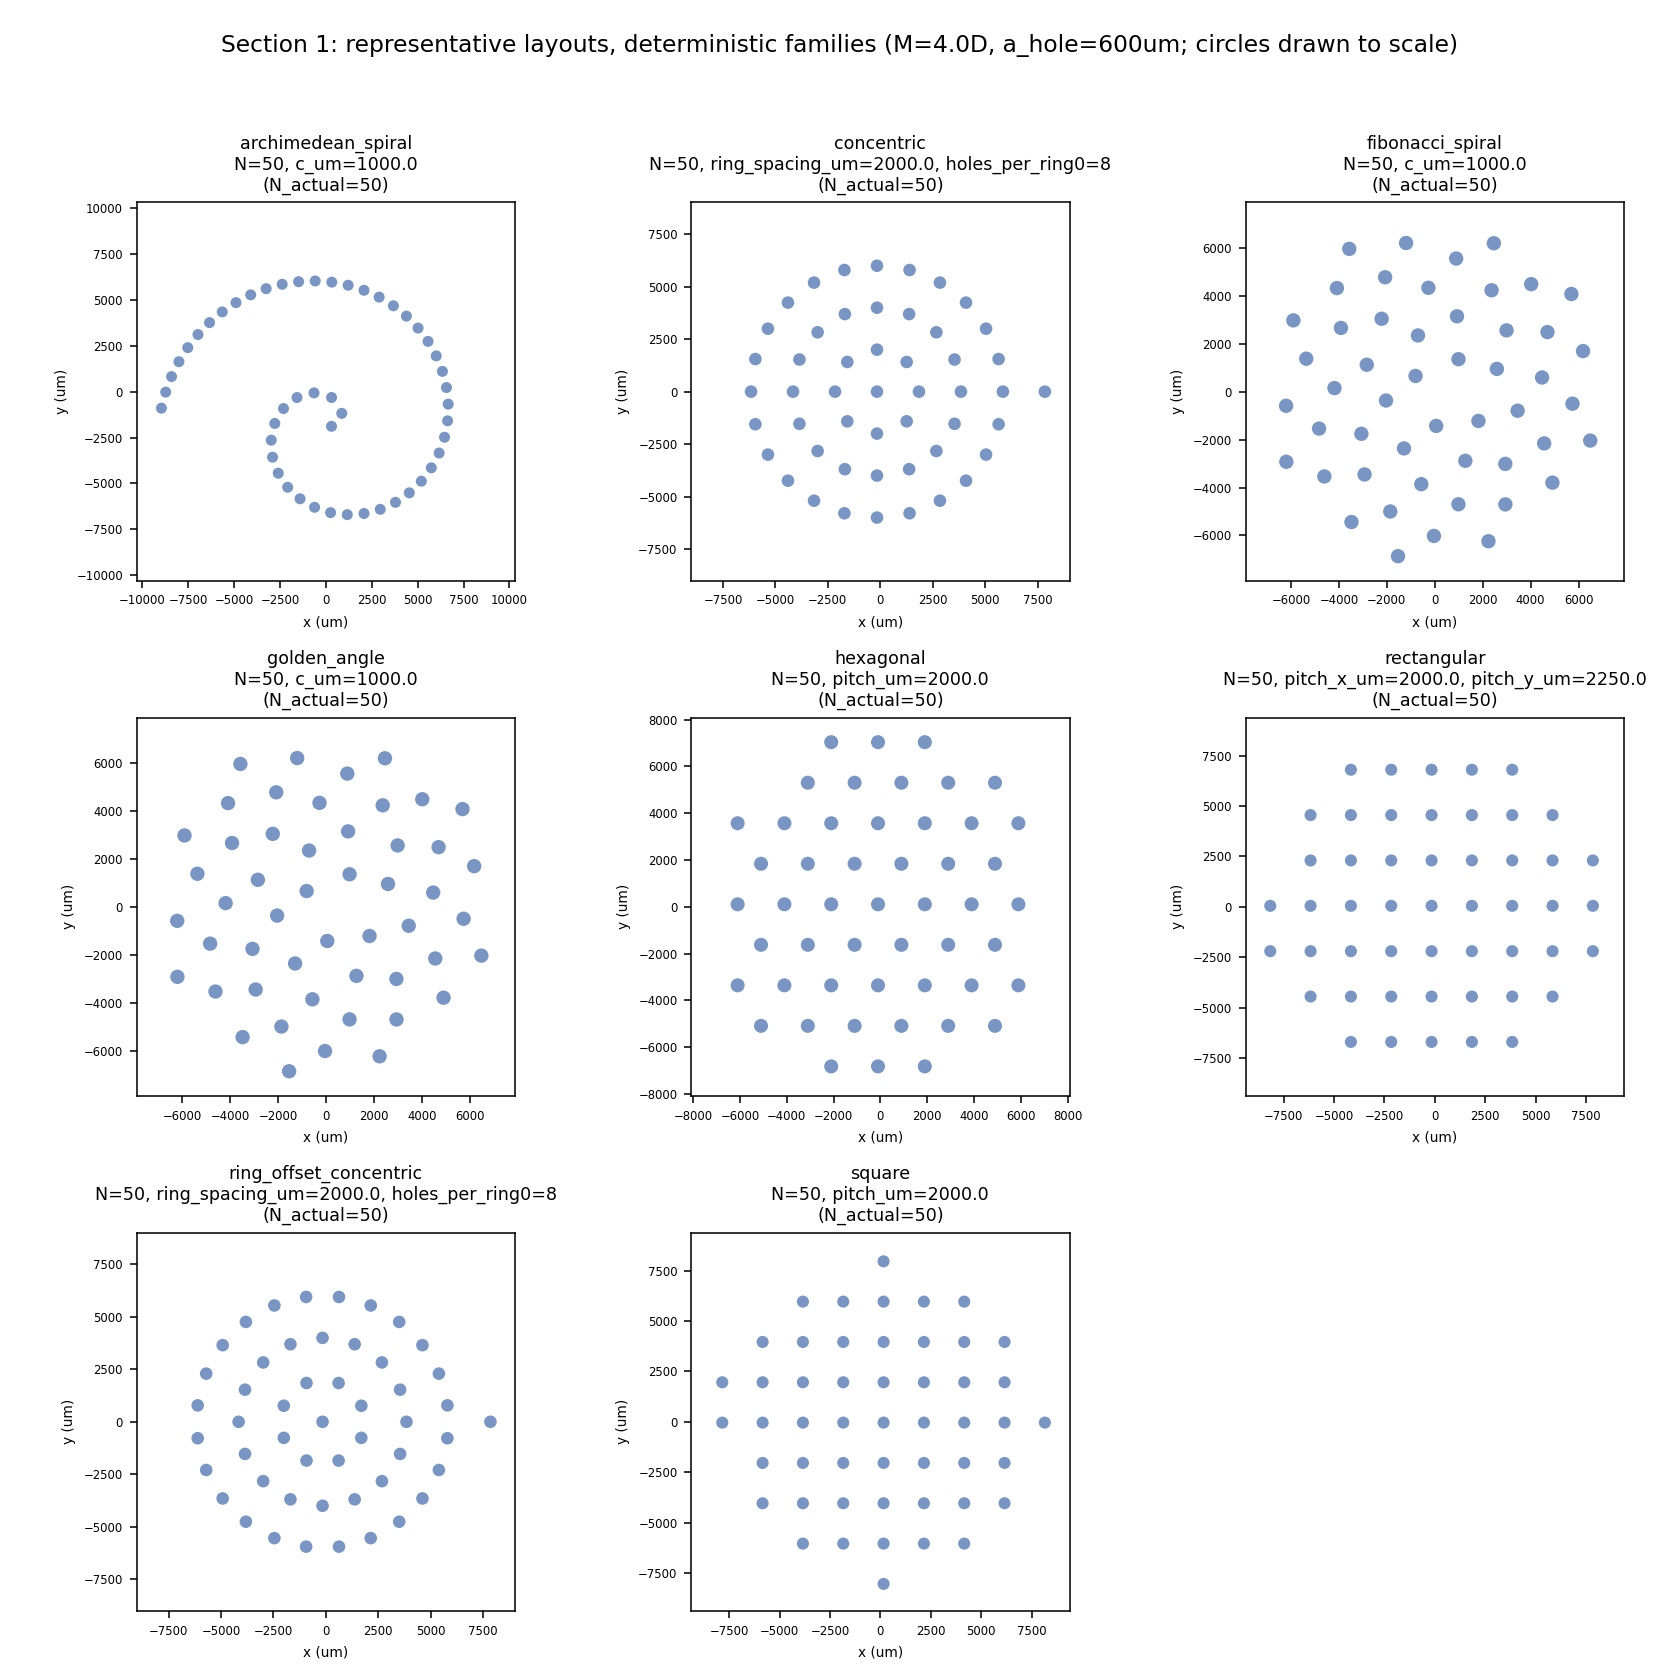
\includegraphics[width=0.95\textwidth]{handbook_figs/section1_deterministic_catalog.png}
\caption{Representative generated layouts for the five deterministic
families, drawn to scale (hole radius shown as filled circles, not just
points) so packing density is visually honest.}
\end{figure}

\begin{figure}[h]
\centering
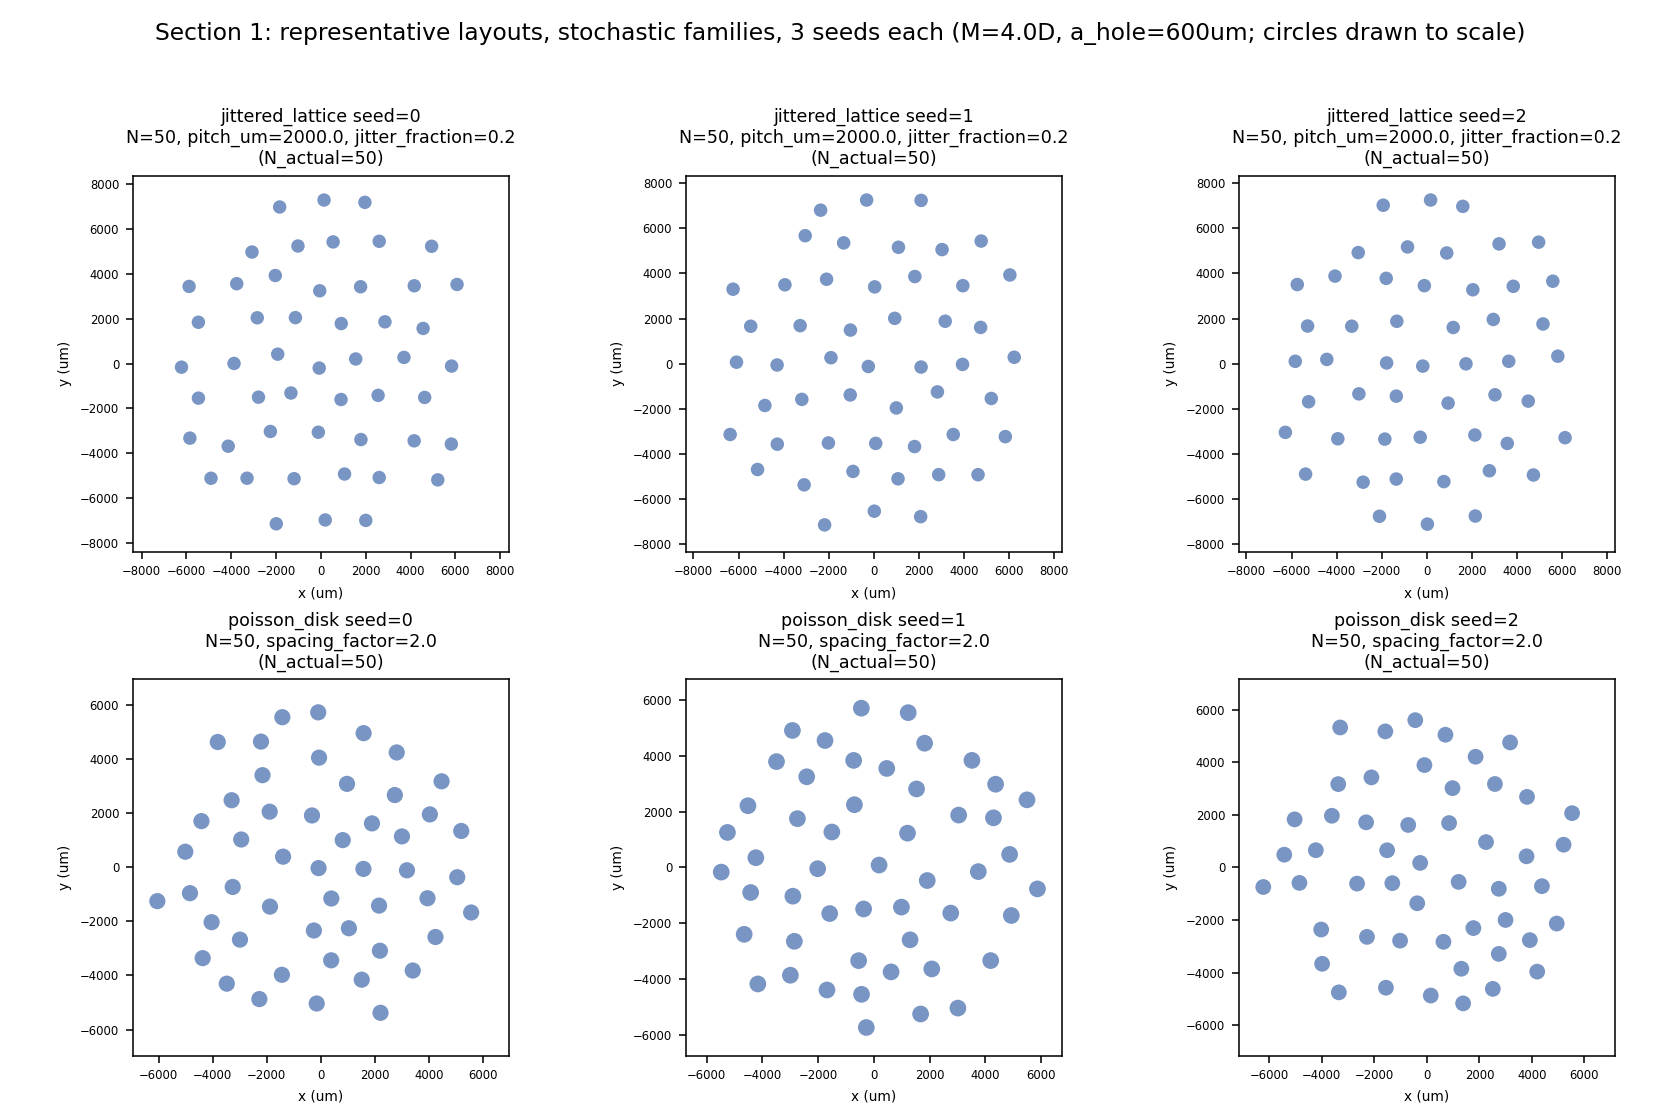
\includegraphics[width=0.95\textwidth]{handbook_figs/section1_stochastic_catalog.png}
\caption{Three different random seeds for the two stochastic families,
shown side by side. The visible differences between seeds are exactly why
these families need seed-averaged safety checking rather than a single
evaluation.}
\end{figure}

\codemapbox{Every geometry family is a small, self-contained function in
\texttt{array\_geometry\_lab/generators/}, one file per family, all sharing
one interface: given a requested hole count and spacing, return a list of
hole-center coordinates. Every generator also rejects (or removes) any hole
placement that would physically overlap its neighbors --- a fabrication
constraint separate from and prior to the optical safety checks. This
overlap-rejection can be aggressive: one documented test case showed a
requested 50 holes collapsing to only 9 actual holes once overlap was
enforced, at a spacing too tight for that hole size.
}
\newpage
